% !TEX TS-program = pdflatex
% !TEX encoding = UTF-8 Unicode

% This is a simple template for a LaTeX document using the "article" class.
% See "book", "report", "letter" for other types of document.

\documentclass[11pt]{article} % use larger type; default would be 10pt

\usepackage[utf8]{inputenc} % set input encoding (not needed with XeLaTeX)

%%% Examples of Article customizations
% These packages are optional, depending whether you want the features they provide.
% See the LaTeX Companion or other references for full information.

%%% PAGE DIMENSIONS
\usepackage{geometry} % to change the page dimensions
\geometry{a4paper} % or letterpaper (US) or a5paper or....
% \geometry{margin=2in} % for example, change the margins to 2 inches all round
% \geometry{landscape} % set up the page for landscape
%   read geometry.pdf for detailed page layout information

\usepackage{graphicx} % support the \includegraphics command and options

% \usepackage[parfill]{parskip} % Activate to begin paragraphs with an empty line rather than an indent

%%% PACKAGES
\usepackage{booktabs} % for much better looking tables
\usepackage{array} % for better arrays (eg matrices) in maths
\usepackage{paralist} % very flexible & customisable lists (eg. enumerate/itemize, etc.)
\usepackage{verbatim} % adds environment for commenting out blocks of text & for better verbatim
\usepackage{subfig} % make it possible to include more than one captioned figure/table in a single float
% These packages are all incorporated in the memoir class to one degree or another...

%%% HEADERS & FOOTERS
\usepackage{fancyhdr} % This should be set AFTER setting up the page geometry
\pagestyle{fancy} % options: empty , plain , fancy
\renewcommand{\headrulewidth}{0pt} % customise the layout...
\lhead{}\chead{}\rhead{}
\lfoot{}\cfoot{\thepage}\rfoot{}

%%% SECTION TITLE APPEARANCE
\usepackage{sectsty}
\allsectionsfont{\sffamily\mdseries\upshape} % (See the fntguide.pdf for font help)
% (This matches ConTeXt defaults)

%%% ToC (table of contents) APPEARANCE
\usepackage[nottoc,notlof,notlot]{tocbibind} % Put the bibliography in the ToC
\usepackage[titles,subfigure]{tocloft} % Alter the style of the Table of Contents
\renewcommand{\cftsecfont}{\rmfamily\mdseries\upshape}
\renewcommand{\cftsecpagefont}{\rmfamily\mdseries\upshape} % No bold!

%%% END Article customizations

%%% The "real" document content comes below...

\title{Exploration of a Lock-Free Hash Table}
\author{Trevor Absher, Martin Dinkov}
%\date{} % Activate to display a given date or no date (if empty),
         % otherwise the current date is printed 

\begin{document}
\maketitle

\section{Abstract}

This paper expands upon an agorithm presented in \textit{Dynamic-Sized Nonblocking Hash Tables} by Liu et. al. A specialization of this algorithm lies in its ability to dynamically resize in both directions. This ability is achieved through a freezable set abstraction that expands upon the standard set operations. A freeze method prevents any thread from editing a given bucket during the hash table resizing process.

We focus on the lock-free version of the hash table, using C++ to implement it. A minor difference lies in the fact that our implementation uses a Linked-List based set. The authors used a single flat array for its benefits regarding cache locality. However, an array-based implementation requires additional bookkeeping to avoid fragmentation. Our lock-free linked list Set implementation is derived from \textit{The Art of Multiprocessor Programming} by Herlihy and Shavit.

The idea of freezing the hash set relies on a resizing operation, dictated by a heuristic policy. The original paper does not cover any preferred heuristics. Thus, we compare the application of various commonly used policies. We also implement a transactional variant of a sequential hash table for the purpose of comparing it to our lock-free concurrent implementation. Our testing for each solution is done across varying hardware architectures in order to explore the solution's portability.

\section{Categories and Subject Descriptors}

D.1.3 [\textbf{Programming Techniques}]: Concurrent Programming -- \textit{Parallel Programming;} E.2 [\textbf{Data Storage Representations}]: Hash-table Representation

\section{Implementation \& Architecture}

\subsection{Freezable Set}

The Freezable Set class (FSet) serves as a wrapper layer around the Set class. The FSet object contains \textit{set} and \textit{ok} variables and defines the FSetOp struct. The \textit{ok} variable is a single bit representing whether or not the FSet is frozen. If \textit{ok} is set to false, then \textit{set} becomes immutable and no threads can add or remove an element. Threads can still check if an element is in the frozen set and retrieve it; which is important for the \textit{InitBucket} method of our HashTable, which will repopulate the current head node's buckets with the data from the previous head node.

The \textit{HasMember} method solely exposes the \textit{Contains} call of the underlying \textit{Set} class. The \textit{Invoke} method triggers either an add or remove operation. This method checks if this operation has not already been completed and if it is a valid operation. After those conditions are met, either \textit{Set::Insert()} or \textit{Set::Remove()} is called dependind on the \textit{op.type} variable; which is set to an enum of either \textbf{INSERT} or \textbf{REMOVE}. The \textit{Freeze} method is simple, yet crucial to the functionality of making the hash table lock free. We made no changes to the Freeze method provided by [1].

A size variable is added to the FSet class as an aide for one of the explored hash table resizing heuristic policies. This variable is only an estimate of the size of the set since it is modified past the linearization point of an \textit{Insert} or \textit{Remove} operation. Implementing a more accurate size query requires use of descriptor objects within the Set class. Descriptors would lead to unneccessary overhead since such size accuracy is not necessary solely for the purpose of determining when to resize.

\subsubsection{FSetOp}

The FSetOp struct contains an enumeration with two values \textbf{INSERT} and \textbf{REMOVE} set to true and false respectively. The \textit{key} variable represents the integer that is going to be either added or removed. The \textit{done} bit is an atomic variable that represents if this specific add/remove operation has already been completed. The \textit{resp} bit is an atomic variable that represents if the operation was successful or not. The operation might fail if an add attempts to add a duplicate value, or if a remove attempts to remove a value that is not in the set. These variables are atomic to ensure all threads see the same statuses of these operations. The \textit{GetResponse} method retrieves the \textit{resp} variable of the object.

\subsection{Set}

The authors of [1] use an array-based set for the core of their bin implementation. However, they do not go into the details of their Set implementation since it is irrelevant to the lock-free hash table algorithm. We use a linked-list based Set class to represent the integer set of the FSet object based on the lock-free version of the Set object given in \textit{The Art of Multiprocessor Programming} [3]. The lock-free Insert and Remove operations provided by this algorithm are necessary to maintain the lock-free property of the hash table. Our chosen Set algorithm also provides a wait-free Contains operation, which is the operation most commonly used in a data structure. The values contained within the Nodes are unique integers and ordered, thus also serving as keys to Node objects in our implementation.

The Set class supports two traversal methods. Set::Find is used for internal traversal within the Set::Insert and Set::Remove calls in order to provide a window of two nodes. The Set::Find method can also plays a part of a lazy removal process. It physically removes any Nodes that have been logically flagged for removal. The logical removal flag is embedded within the first bit of the pointer that links the Node. Bit-stealing is used in order to avoid the overhead of using a descriptor object and to maintain linearizability. The physical deletion is done using a CAS call. If this CAS call fails, then a neighboring Node must have been inserted or removed and the traversal must start over from the first sentinal Node. Such failure denotes that another thread must be making progress.

Set::Contains provides the other traversal method, which always traverses each Node once and linearizes in a deterministic amount of steps. This deterministic quality of Set::Contains guarantees wait-freedom. The Set::Contains method linearizes once it has found a Node that has a value that is NOT less than the value that is being queried. If the first such value found is greater than the value queried, then the value queried is not in the Set since the Nodes are ordered based on their values.
 
The Set::Remove method obtains a Set::Window of two Nodes using Set::Find based on the value that is to be removed. If the second of these Nodes has a value different from the one to be removed, then the value to be removed does not exist in the Set and the Set::Remove call fails and returns false. Alternatively, if the value to be removed is found, then the corresponding Node is logically flagged for deletion using a CAS call. Similarly to the physical removal in Set::Find, failure of this CAS call denotes that a another thread has made progress by inserting or removing a neighboring Node. In such case of this CAS failure, the Set must be re-traversed from the beginning. A logical deletion is attemped using CAS call following the physical deletion. It is okay for this second CAS to fail as the Node will be physically deleted in the following Set::Find call.

The Set::Insert method also obtains a Set::Window of two Nodes, similarly to Set::Remove. If the value of the latter of the Nodes is equal to value being inserted, then the value already exists and the Set::Insert call fails by returning false. Otherwise, the value is inserted between the two Nodes from the Set::Window object. A new Node is created using the value being inserted. This Node is inserted using a CAS call. If the CAS call happens to fail, it is only due to another call making progress and the Set must be retraversed once again.

The original algorithm provided by Herlihy and Shavit [3] is extended with the implementation of the \textit{Set::Union} and \textit{Set::IntersectionRemainder} methods. Such methods are utilized for the binary resizing capability of the housing hash table class. A Set::Union call is provided with another Set as an argument, which is combined with the Set instance upon which the method is called. The Set::IntersectionRemainder iterates through the Nodes of the Set instance upon which the method was called and picks any Nodes that meet a criteria into a new Set. The criteria is that the value of the Node must have a given remainder when divided by a given divisor. Both of the aforementioned methods do not require thread-safe properties because they are only called once parenting FSet class has been frozen and no further modifications to the Set can be made.

\subsection{Hash Table}

As most hash tables, this one's public interface supports three methods: \textit{Insert}, \textit{Remove}, and \textit{Contains}. The pseudocode for these methods are specified in [1]. This HashTable implementation can house up to two internal hash tables, which are referred to HNodes in [1]. Having up to two HNodes allows for the unique resizing properties of this lock-free data structure. Below are two critical distictions between the HNodes:
The first HNode must always be present and is accessed via a head HNode member pointer. The second HNode can be accessed through the \textit{pred} pointer of the first HNode and is non-existant if that pointer equals NULL. The HNode pointers are atomic variables since they can be accessed by multiple threads.
The first bin can have un-initialized (NULL) bins. The second HNode is used to initialize the bins of the first HNode. All bins of the second HNode MUST be initialized and cannot be NULL. A third HNode is not present to initialize the bins of the second HNode.

Set::Resize is an internal call that can be triggerred by an Insert or Remove based on a heuristic policy. The heuristic policy choise can significantly impact performance. Set::Resize should'nt be called too often since the Set::Resize call is expensive. However, Set::Resize should be called often enough so that the bin sizes do not become too large, which would result in expensive traversals. In an effort to avoid the overhead of two threads attempting to resize simultaneously, the atomic bool flag m\_resizing is introduced, which was not included in [1]. Resize can only be called if a CAS call successfully flips the flag from false to true. Once resizing procedure is complete, m\_resizing is set back to false via an atomic write.

The implementation of Set::Resize initializes all of the bins in the first HNode that have not already been initialized. A new HNode is created with a number of bins equal to double or half of the bins in the first HNode. The current first HNode is set as the pred pointer of the newly created HNode in preparation to make it a second HNode and the newly created HNode is set as the first HNode using a CAS call. If the CAS fails, it is only due to another Set::Resize call (triggerred by another Insert or Remove) successfully executing its resize. Since the HashTable has been resized even when the CAS fails, the CAS call does not need to be reattempted. This CAS call represents the linearization point of the resizing functionality of the HashTable. No bins are initialized in the first HNode immediately following a resize. Instead, the work for initializing the bins in the first HNode is distributed amongst the future calls that access those bins.

The Set::InitBucket method is used to populate a NULL bin in the first HNode. During this call, the NULL bin is populated with data from the second HNode, which is always initialized. The second HNode can either have half or double the size of the first HNode, denoting whether the last Set::Resize call grew or shrunk the hash table. If the table has been shrunk, then bin N in the first HNode inherits the values of bin N and N + numBins1 (where numBins refers to the number of bins in the first HNode). The proccess is slightly more convoluted if the table has grown. For such cases, bin N in the first HNode is populated with the entries in bin N \% numBins2 that have a remainder of N when divided by numBins1. The bins in the second HNode are always frozen prior to being accessed. The Set::InitBucket method is linearizable since the bin pointers in the HNode object are atomic and a CAS call is used to replace a NULL bin with a newly created one. That CAS also represents the linearization point of the initialization of a bin. The call can only fail if another call has came through and initialized that same bin, thus making it unnecessary to retry again.

The Set::Apply method represents a private helper function for processing an Insert or Remove. Apply can only be called on a bin in the first HNode. The designated bin is initialized if it happens to be NULL. An Insert or Remove should never fail due to a bin being frozen because only bins in the second HNode can be frozen. Each Insert or Remove call linearizes once it reaches the previously discussed linearization points within the underlying Set class. A size member (similar to the one in FSet) is implemented in the HashTable class, which is not part of the pseudocode in [1]. This variable is atomically incremeneted and decremented upon successful Insert and Remove operations. Again, this is only an estimate of the total number of nodes in the table and solely used as part of a resizing heuristic policy.

Set::Contains is the only other operation (besides InitBucket) that can access the bins within the second HNode, even if they happen to be frozen. Contains can collide with a Set::Union or Set::IntersectRemainder call, but that is acceptable because all of these functions only perform read operations on the Set class. Since Set::Contains does not have to initialize any bins, it is much more lightweight than a Insert or Remove. If Set::Contains had the ability to initialize bins, that would also significantly increase the contention on the InitBucket call since Contains is statistically more common than any other operation. The Contains call can complete in a prederminite number of steps even within the higher wrapping classes, thus maintaining the wait-free behavior that is introduced in the underlying Set class.

\section{Concurrency}

\subsection{Progress Guarantees}

Since our entire implementation is lock-free, at least one thread is guaranteed to make progress at any time. All finalized changes done to either the head node or its buckets are done using atomic CAS calls. If a thread fails to successfully update a value by failing the CAS call, it is only due to the fact that the value it expected was changed by another thread. In such cases, the other thread's CAS call must have succeeded. The concurrent behavior of each CAS call is explained in the Implementation section on a case-by-case basis. Generally, a successful CAS call represents the linearization of the parent function. Therefore, if another thread has linearized, it is making progress.

The Contains functionality of our implementation also provides wait-freedom, which is a stronger guarantee than lock-freedom. Each layer of a Contains call can execute in a predeterminant amount of steps, mostly depending on the number of Nodes that have to be traversed. Having a wait-free Contains that does not depend on CAS calls also helps decrease contention on shared data. The local InitBucket and Resize calls also provide wait-free progress because they do not require iterative CAS calls. As mentioned earlier, their CAS calls can only fail if another thread came through and already executed the same operation.

\subsection{Correctness Conditions}

All of the operations supported by our HashTable class and its subclasses are linearizable. Therefore, each operation has a single linearization point. Each linearization point is discussed on a case-by-case basis in the Implementation section. For most cases (with the exception of Contains), the linearization point is represented by an atomic CAS call. The thread locally processes a structure and utilizes the atomic CAS call to make that structure resident to all other threads. The order of all overlapping operations is determined by the point-in-time that each operation linearizes. 

\subsection{Synchronization Techniques}

The synchronization techniques in this algorithm are composed of atomic variables and atomic calls, including atomic reads, writes, and CAS calls. Atomic calls are implemented to execute using a single operation that is provided as part of the hardware ISA. Therefore, such operations always execute entirely or not at all. Atomic reads and CAS calls are guaranteed to retrieve the latest version of a variable, which may not be in a local cache. Therefore, having multiple threads calling atomic operations on a variable can thrash the cache and lead to performance losses. Each atomic operation is discussed on a case-by-case basis throughout the Implementation section of this paper.

\section{Profiling}
All profiling data in the scope of this paper is profiled on a Intel i7-7820x based platform, unless "AMD" is included in the title of the data. The AMD chip used is an AMD Ryzen 7 1700. Both CPUs support up to 16 logical threads on 8 physical cores and are manufactured based on a 14 nm process. The Intel and AMD chip run at a base frequency of 3.60 GHz and 3.00 GHz respectively. In that sense, the Intel chip has a slight advantage.

Four data sets of 2000000 operations are used during the profiling runs. A large number of operations was chosen in order to reduce (1) variation introduced by the CPU frequency not being forced to a constant value and (2) overhead due to thread creation and destruction. All data sets are generated using the attached genHashTableData Python script. The four data sets vary based on (1) the range of values used as arguments and (2) the proportions of operation occurrences.

\begin{itemize}
	\item InsRem-50-64K.dat
	\begin{itemize}
		\item Proportions: 50\% Inserts, 50\% Removes, 0\% Contains
		\item Argument Range: 0-64,000 
           \item First 25\% of operations are Inserts in order to pre-load the data structure 
	\end{itemize}
	\item Contains-90-64K.dat
	\begin{itemize}
		\item Proportions: 9\% Inserts, 1\% Removes, 90\% Contains
		\item Argument Range: 0-64,000 
           \item First 5\% of operations are Inserts in order to pre-load the data structure 
	\end{itemize}
	\item InsRem-50-256.dat
	\begin{itemize}
		\item Proportions: 50\% Inserts, 50\% Removes, 0\% Contains
		\item Argument Range: 0-256
           \item First 25\% of operations are Inserts in order to pre-load the data structure  
	\end{itemize}
	\item Contains-50-256.dat
	\begin{itemize}
		\item Proportions: 9\% Inserts, 1\% Removes, 90\% Contains
		\item Argument Range: 0-256
           \item First 5\% of operations are Inserts in order to pre-load the data structure  
	\end{itemize}
\end{itemize}


\subsection{Resizing Heuristic Policy}

Determining when to resize and how often the resizing operation is done can significantly impact the performance and scalability of the algorithm. As a result, different heuristic policies are profiled in order to try to maximize the performance and scalability. The policies are based on the size and (upper/lower) threshold members found in the HashTable and FSet classes.

The original paper suggests to grow the number of bins when the bin being accessed becomes too large and to shrink whenever a random sample of bins are too small. A bin becomes too large when the number of values it contains exceeds the upper threshold value. Alternatively, a bin is too small when it has less values than the lower threshold value. Gathering a random sample of bins can get expensive due having to access multiple atomic values on a per-bin basis.

We explored a slight variation of the policy suggested by the authors. In our policy, downsizing is based on the size of the current bin being accessed, instead of a random set of bins. The data below shows the observed execution times when using this heuristic.

\bigskip
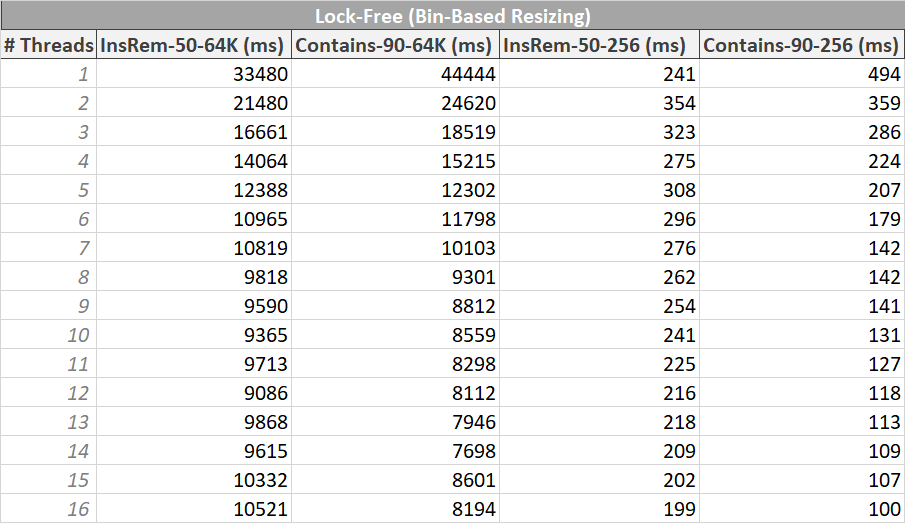
\includegraphics[width=0.5\linewidth]{TableA.png}
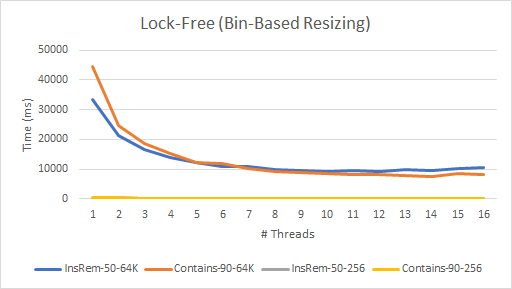
\includegraphics[width=0.5\linewidth]{GraphA.png}

Reoccurring operation arguments are less likely in the datasets that have an argument range up to 64K. For such cases, the Insert and Remove operations are more likely to succeed and check the heuristic policy. The long execution times for these data sets are due to the resize method being called too often. Consecutive resize calls are being made because the size of the bins are not uniform.

We came up with an alternative heuristic that is agnostic to how uniform the sizes of the different bins are. This heuristic tracks all of the values in the hash table as a whole, instead of the size of the individual bins. This heuristic also introduces dynamic thresholds that do not require user input. The lower threshold is always equal to the number of bins in the hash table. This denotes that a single entry exists in each bin on average. The upper threshold is a multiple greater than two of the number of bins. Having a multiple greater than two is critical in order to avoid resizing in two consecutive operations. Various values for the multiples are profiled in the data included in the Appendix section. The data from the optimal multiple for our data set is shown below, which proved to be 64.

\bigskip
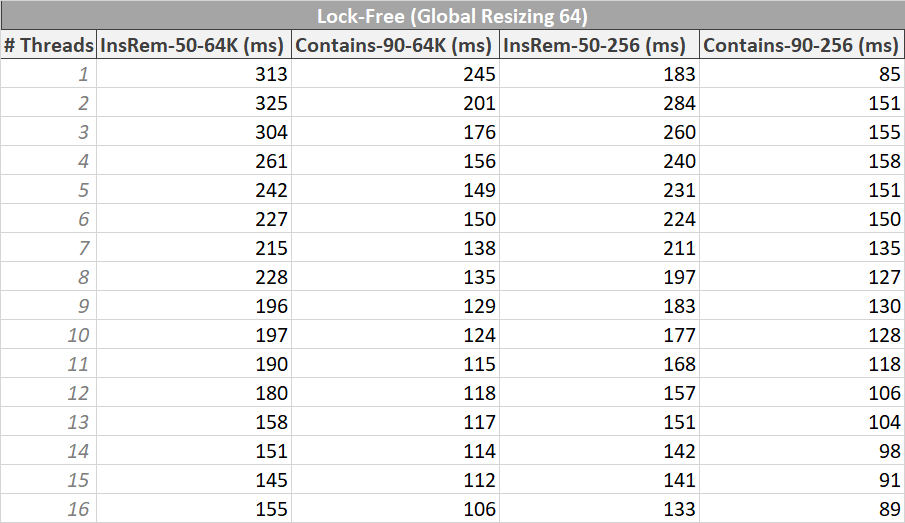
\includegraphics[width=0.5\linewidth]{TableF.png}
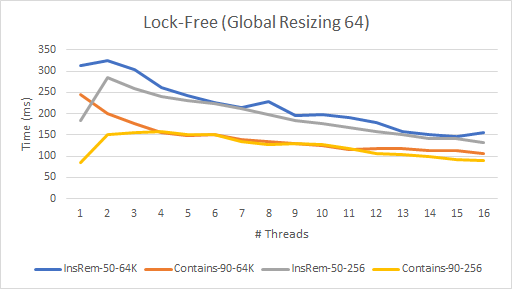
\includegraphics[width=0.5\linewidth]{GraphF.png}

\section{Transactional Implementation Using STM}

Software Transactional Memory (STM) libraries allow atomicity to be implemented in software for a set of operations, known as a transaction. Each transaction must be entirely executed or not at all. Such behavior requires rewinding functionality that allows all the progress made by a transaction up to a certain point to be undone if another transaction has overwritten data shared between the two transactions. Rewinding a transaction can introduce additional overhead that is not present within other methodologies. Nevertheless, if a transaction is being rewound, it is due to another transaction making progress.

\subsection{Sequential Hash Table}

STM allows for a sequential implementation of a data structure to be made concurrent by defining its operations as transactions. In fact, the implementation must be sequential because the STL atomic operations fail to compile if they are defined within a GCC STM transaction. This section covers the implementation of the sequential hash table, which mimics the lock-free version but without the thread-safety functionality.

Two different implementations for the hash table bins are explored. One implementation (Sequential::Set class) utilizes a binary search tree for its quick logarithmic-time search functionality. The other implementation utilizes a linked-list (Sequential::List) for its ability to be easily split into two lists or combined with another list into a single one. The benefit of using the List class for the bins is only apparent if the hash table supports proper resizing hierarchy. Without proper resizing, the bins may grow too large and in which case the linear search time of the List make it inferior to the Set.

In addition to the traditional Insert, Remove, and Contains operations, the Set and List classes also include a Union and IntersectRemainder operations. Just like in the lock-free hash table, they are used when resizing the number of bins. Union combines two bins together while IntersectRemainder splits a bin into two based on the remainder value when dividing each element. These operations are simplified in the List implementation because:

\begin{itemize}
	\item An existing list can be recycled
	\begin{itemize}
		\item During a Union, the elements of the shorter List are inserted into the longer list.
	\end{itemize}
	\item Since both Lists are always sorted, each of these operations require a single traversal through each List resulting in an O(m+n) complexity.
	\begin{itemize}
		\item On the other hand, the time complexity of equivalent calls in Set is O(m * (n * log(n))) since each the tree has to be re-traversed for each Insert.
	\end{itemize}
\end{itemize}

A set of verification tests are included in Tests.h that check the correctness of the Set and List classes. This code can be triggered by running the SequentialHashTable executable with an invalid set of parameters.

The InsRem-50-64K data set is used to compare the different variants of the Sequential::HashTable since it is the most stressful. The single-threaded results are shown below, which confirm the differences between the Set and List implementations.

\begin{itemize}
	\item Sequential::Set is used for bin implementation and resizing is DISABLED.
	\begin{itemize}
    		\item 195ms
	\end{itemize}
	\item Sequential::Set is used for bin implementation and resizing is ENABLED.
	\begin{itemize}
		\item 118ms
	\end{itemize}
	\item Sequential::List is used for bin implementation and resizing is DISABLED.
	\begin{itemize}
		\item 6494ms
	\end{itemize}
	\item Sequential::List is used for bin implementation and resizing is ENABLED.
	\begin{itemize}
		\item 100ms
	\end{itemize}
\end{itemize}

From here on, Sequential::List is used with resizing enabled. Various resize hierarchies are explored in this implementation, as for the lock-free hash table. Resizing based on the cumulative number of entries in the hash table again proves to be more efficient than resizing based on the size of individual bins. Resizing based on individual bins can lead to the number of bins constantly fluctuating if one bin has a lot of entries and another bin has very few. The lower threshold was chosen to be equal to numBins, since the optimal upper threshold showed to be 4 * numBins. Having thresholds that are > 2 times apart eliminates the possibility of resizing twice in two consecutive operations.

\begin{itemize}
	\item Resizing based on bin size. This can be enabled by changing the “\#if 0” occurrences in Sequential::HashTable to “\#if 1”
	\begin{itemize}
    		\item 170ms
	\end{itemize}
	\item Resizing based on cumulative number of entries in hash table. Upper threshold is set to 2 * numBins. Lower threshold is set to numBins.
	\begin{itemize}
		\item 123ms
	\end{itemize}
	\item Resizing based on cumulative number of entries in hash table. Upper threshold is set to 4 * numBins. Lower threshold is set to numBins.
	\begin{itemize}
		\item 100ms
	\end{itemize}
	\item Resizing based on cumulative number of entries in hash table. Upper threshold is set to 8 * numBins. Lower threshold is set to numBins.
	\begin{itemize}
		\item 109ms
	\end{itemize}
\end{itemize}

\subsection{One Operation Per Transaction}

The GCC transactional memory library is used in this implementation instead of RSTM because GCC is more commonly used and thus more likely to be streamlined. Also, the GCC transactions are implemented at the compiler level and are thus likely to be more efficient. Initially, each Sequential::HashTable operation is wrapped in its own transaction using the \_\_transaction\_atomic compiler directive. This compiler directive does not allow the compiler to insert locks, unlike the \_\_transaction\_relaxed directive [4]. SuperMalloc is used in this implementation as well in order to provide thread-safe memory allocations and deallocations. Introducing SuperMalloc did not create a noticeable change in performance.

The table below shows the results of having a single operation per each atomic transaction. The runtime of the single threaded test cases have likely increased due to the overhead of preparing and submitting the transactions. The runtime becomes progressively worse with each additional thread since there are various possibilities for collisions throughout every function. Contains is the only exception, hence why it shows the best performance.

\bigskip
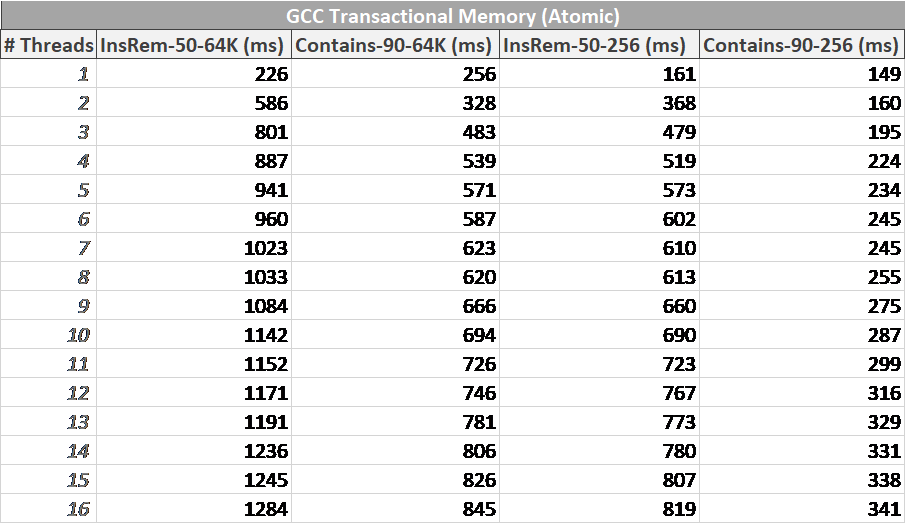
\includegraphics[width=0.5\linewidth]{Table1.png}
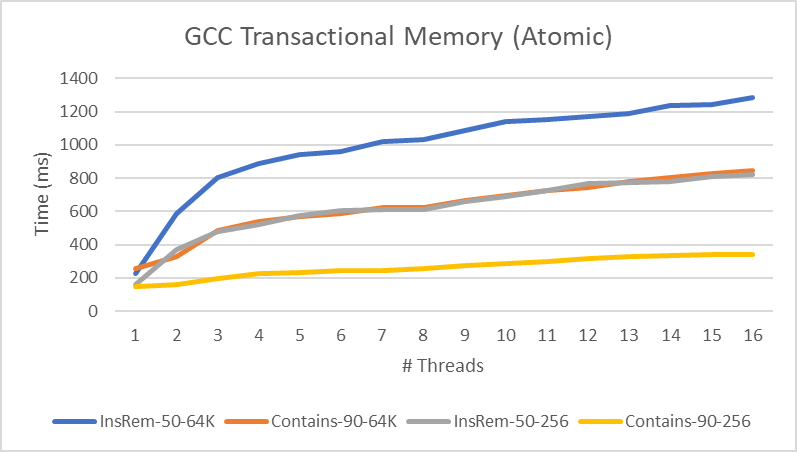
\includegraphics[width=0.5\linewidth]{Graph1.png}

\subsection{Multiple Operations Per Transaction}

Packing multiple operations within a transaction proves to be more efficient for this kind of hash table. Having less transactions overall leads to less overhead dedicated to handling and submitting the transactions. This performance gain is directly reflected in the single-threaded case. However, having longer transactions leads to longer rewind procedures. This is likely why the rate of change drastically increases beyond 8 threads in the charts below, when collisions become much more likely.

The graph below shows the results from having two operations per transaction. This is significantly more performant than having a single operation per thread, since the gain of having to do bookkeeping for less transactions outweighs the loss of the transactions being longer. With more threads, this case is likely to become less performant than having a single operation per transaction.

\bigskip
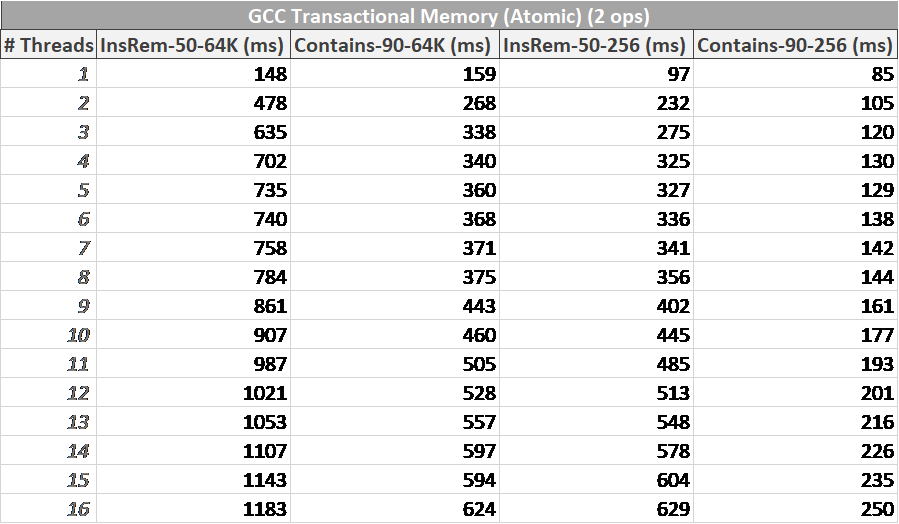
\includegraphics[width=0.5\linewidth]{Table2.png}
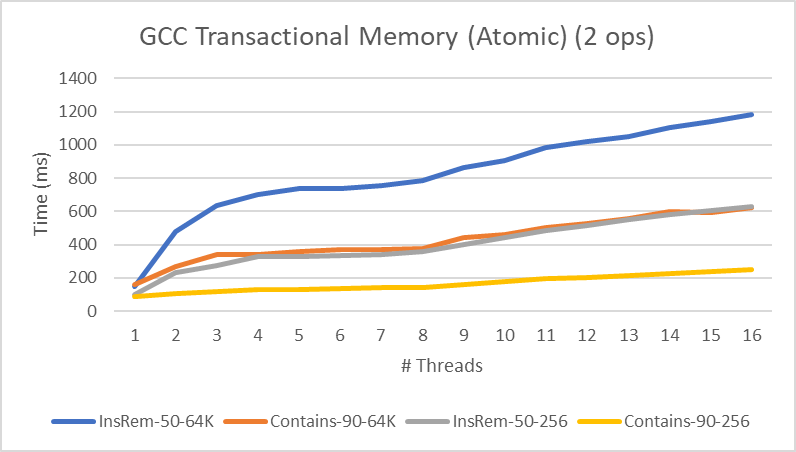
\includegraphics[width=0.5\linewidth]{Graph2.png}

The graph below shows the results from having four operations per transaction. It is more efficient than the either of two previous cases at lower number of threads. However, at higher number of threads it becomes no better than having two operations per transaction.

\bigskip
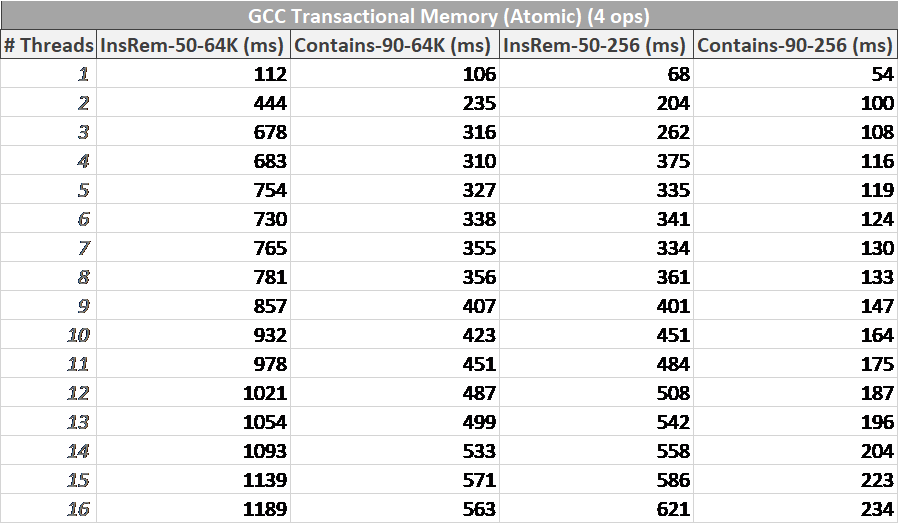
\includegraphics[width=0.5\linewidth]{Table3.png}
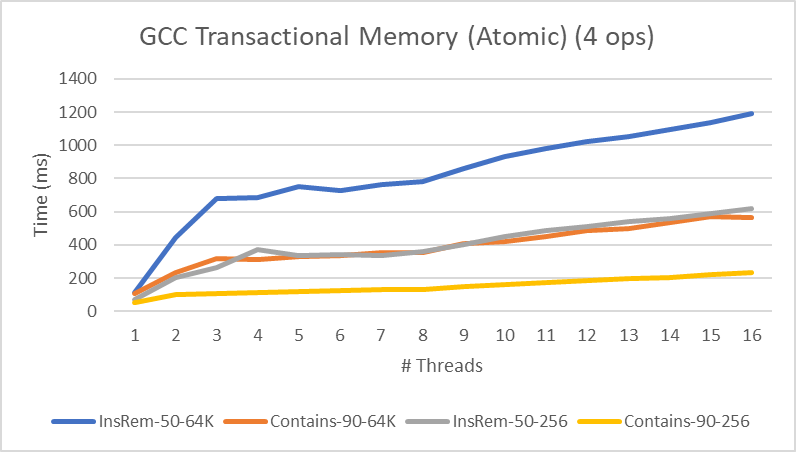
\includegraphics[width=0.5\linewidth]{Graph3.png}

\subsection{Improvement Attempts}

This section covers several attempts to improve upon the STM implementation of the hash table. The only one that proves to be effective is to use coarse-grained locks instead of transactions for this kind of data structure.

\subsubsection{Relaxed Transactions}

Having relaxed transaction instead of atomic ones allows GCC to determine if using locks for some cases can be more efficient than atomicity. Atomicity can become too convoluted to implement in some cases [4]. The data below show the results of using relaxed transactions for the case where a transaction includes only a single operation. It seems no different from the case where the transactions are strictly atomic. The results from having relaxed transactions for the cases where a transaction encompasses multiple operations are also like the ones with strictly atomic transactions.

\bigskip
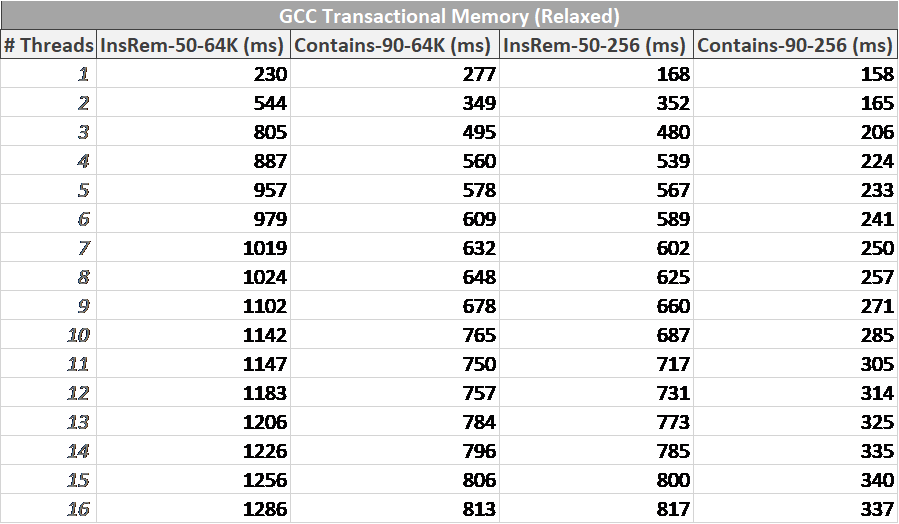
\includegraphics[width=0.5\linewidth]{Table4.png}
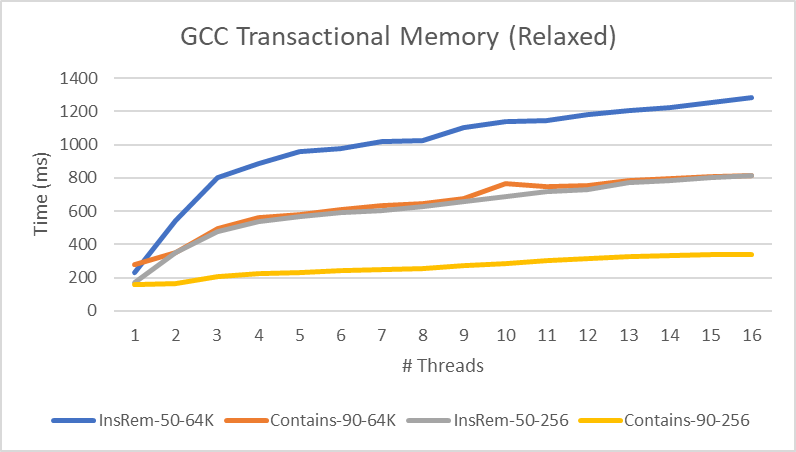
\includegraphics[width=0.5\linewidth]{Graph4.png}

\subsubsection{Replacing Transactions with Locks}

Using locks (via std::mutex) instead of transactions showed approximately 20\% higher performance. Mutexes synchronize the operations, but collisions are eliminated and thus rewinds are no longer necessary. The data below shows the results from wrapping each operation in a mutex. If multiple operations are wrapped, then the performance is likely to be even better since there will be less contention points.

\bigskip
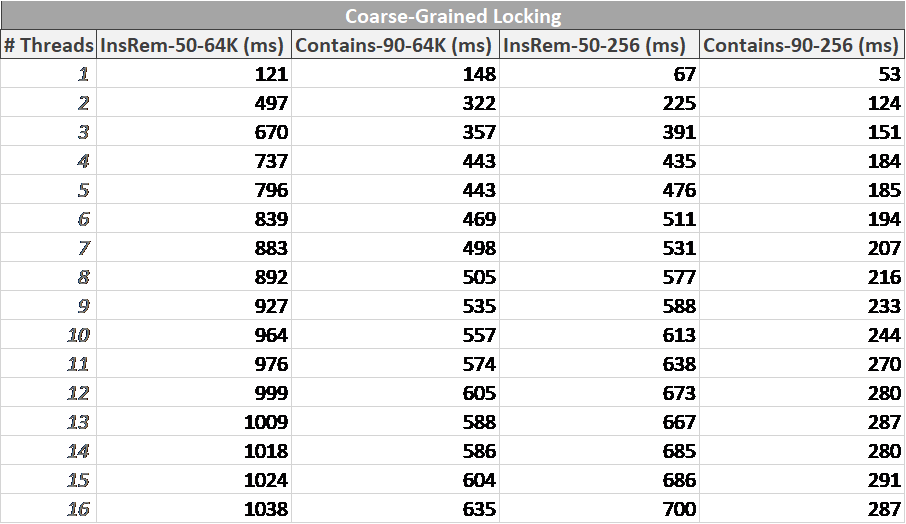
\includegraphics[width=0.5\linewidth]{Table5.png}
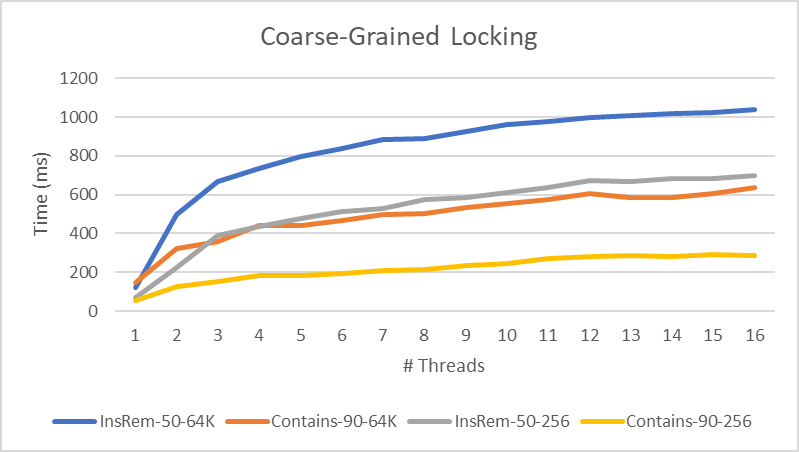
\includegraphics[width=0.5\linewidth]{Graph5.png}

\subsubsection{Offsetting the Transactions}

The synchronize keyword in GCC allows a block of code to always executed sequentially. Under the hood, this is likely implemented using locks and requires that the transactions be relaxed. Wrapping various points of the code to offset the transactions and reduce the number of collisions leads to an increased overall execution time. The collisions likely still occur, and additional overhead is introduced by serializing parts of the code.

\subsection{Comparison to Lock-Free Implementation}

The STM implementation of the Hash Table does not scale well with additional threads, in contrast to the lock-free implementation. The two implementations have comparable performance only when using two threads are being executed. However, the STM implementation is significantly simpler to apply to a sequential data-structure.

\section{Conclusion}

In this paper, we introduced our own implementation of the Lock-Free Dynamic-Sized Nonblocking Hash Tables created by Liu et. al in [1]. Our implementation differed from theirs in a few ways. Our Set object was a linked list as opposed to an array. The underlying Set impementation is not a core aspect of the Hash Table implementation and thus was not discussed in detail by the authors. We also added a resizing heuristic policy that was not part of the original pseudocode. However, we are assuming that the authors implemented their policy in a similar fashion. Multiple policies were explored and profiles, which are discussed in the Resizing Heuristic Policy section.

Re-implementing Liu et. al's data structure was not without its challenges. Converting their pseudocode to functional C++ code was often difficult, especially with certain operations that were not explicitly coding techniques, such as the union operation found in the pseudocode for the FSet object. Implementing the parts of the data structure not described by the authors was also troublesome. Coming up with our own heuristic policies to resize the hash table on took some time and we had to entirely change the Set from operating on an array to operating on a linked list, which involved creating a whole new class with all of its own methods. 

This data structure provides a lot of new advantages to existing alternatives. The biggest its dynamic property; being able to grow and shrink while previous hash table implementations were only able to grow. In an environment with limited memory this data structure is far optimal to its alternatives due to this key feature. It also allows keys to be moved among buckets during a resize operation which previous data structures have not done. Doing this during the resize allows this implementation to avoid sacrificing throughput or progress. Also, the buckets are unbounded and no assumption is made about the size of memory, which allows this data structure to be more flexible in its applications onto larger datasets. While the inner mechanisms of this data structure can be complicated, as there are four encapsulating layers of objects; once it has been successfully implemented the advantages of it far outweigh this.

\section{Appendix}

\bigskip
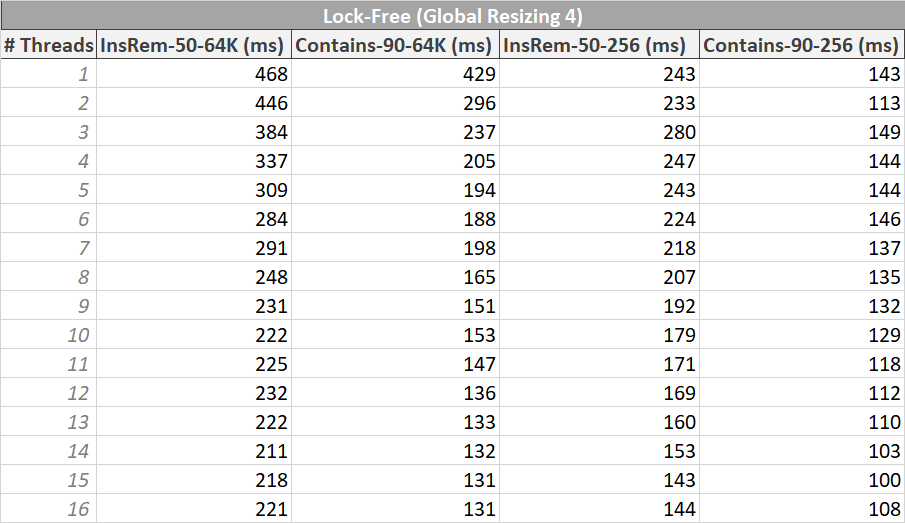
\includegraphics[width=0.5\linewidth]{TableB.png}
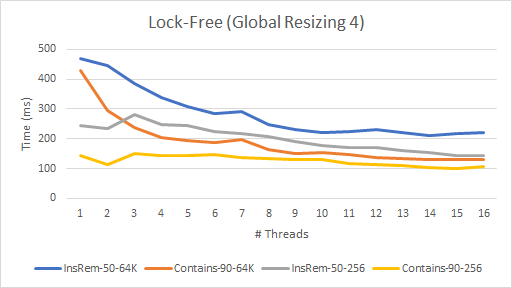
\includegraphics[width=0.5\linewidth]{GraphB.png}
\bigskip
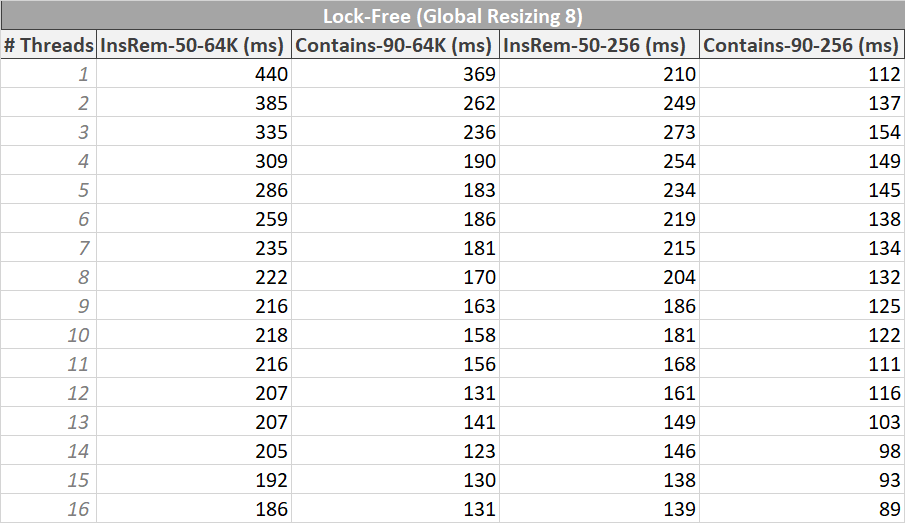
\includegraphics[width=0.5\linewidth]{TableC.png}
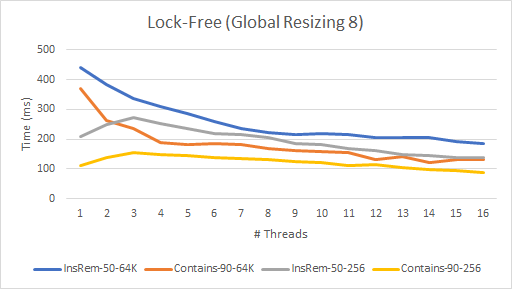
\includegraphics[width=0.5\linewidth]{GraphC.png}
\bigskip
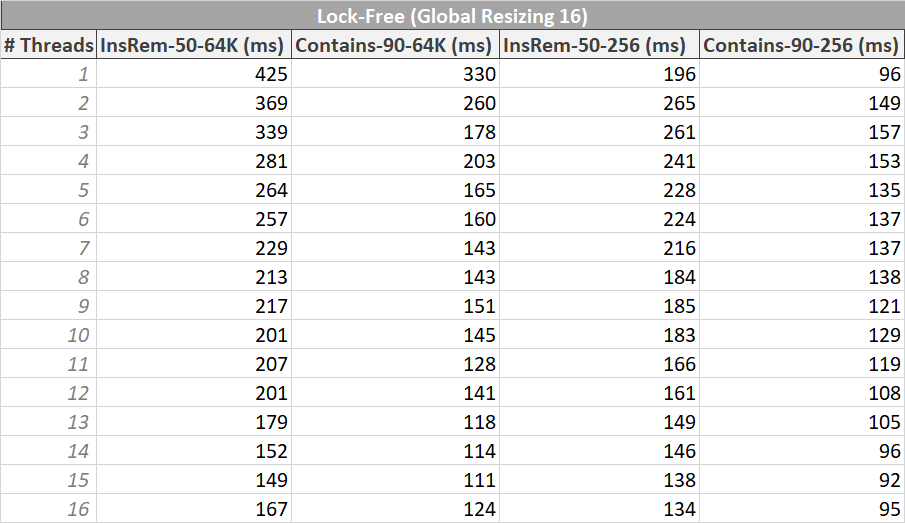
\includegraphics[width=0.5\linewidth]{TableD.png}
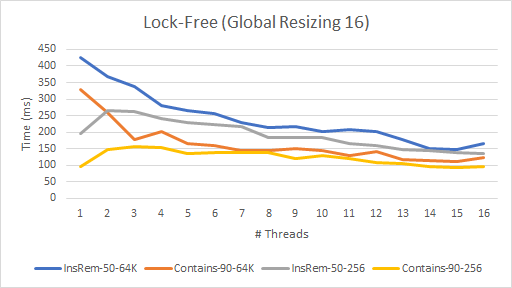
\includegraphics[width=0.5\linewidth]{GraphD.png}
\bigskip
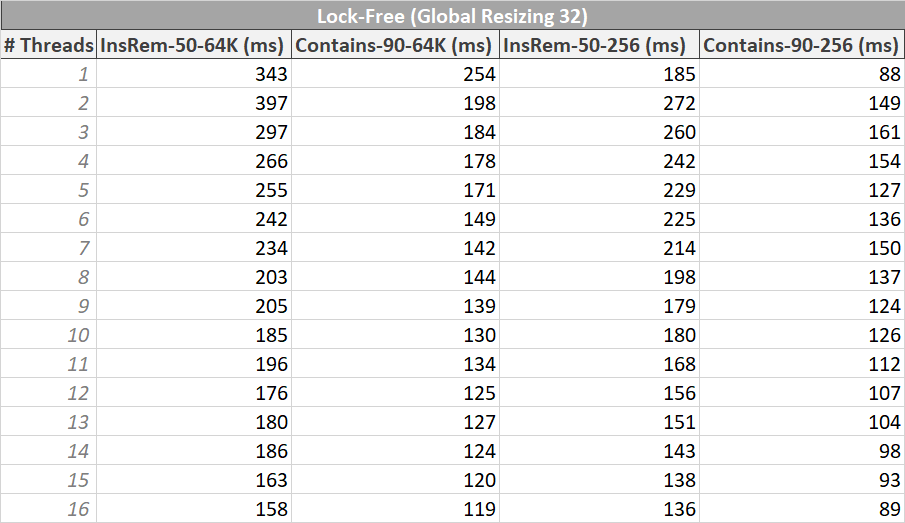
\includegraphics[width=0.5\linewidth]{TableE.png}
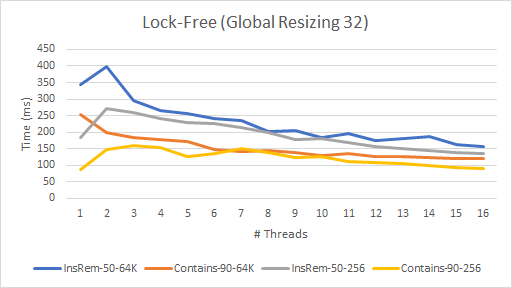
\includegraphics[width=0.5\linewidth]{GraphE.png}
\bigskip
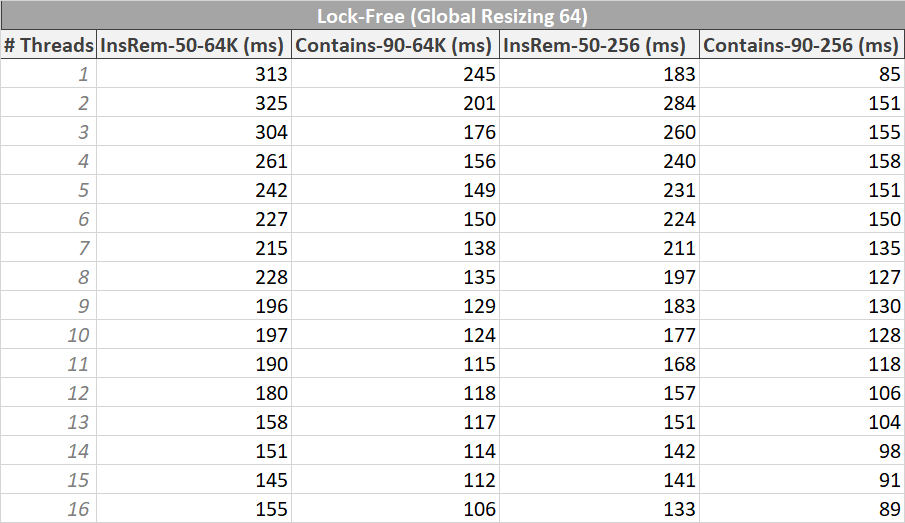
\includegraphics[width=0.5\linewidth]{TableF.png}
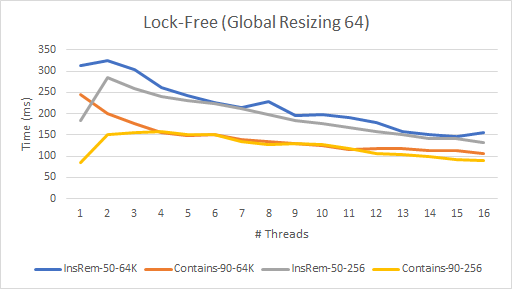
\includegraphics[width=0.5\linewidth]{GraphF.png}
\bigskip
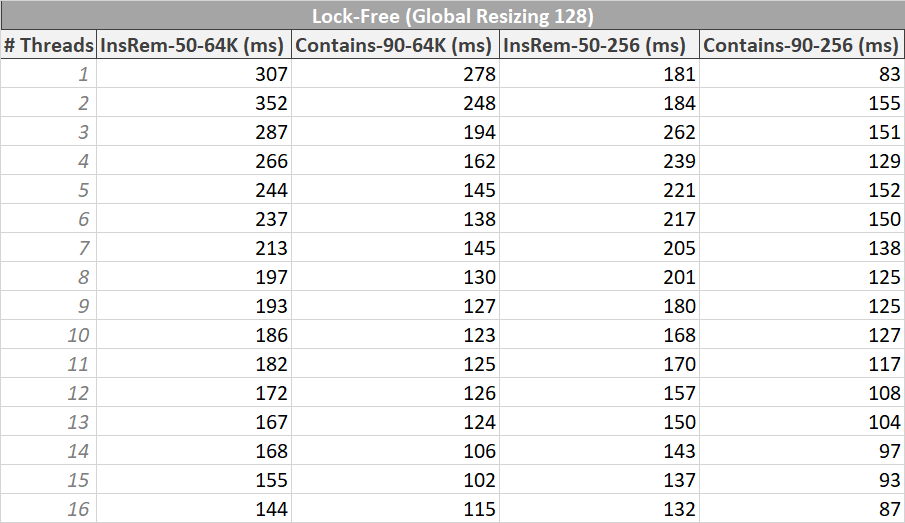
\includegraphics[width=0.5\linewidth]{TableG.png}
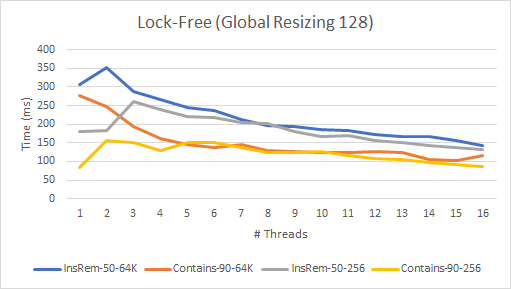
\includegraphics[width=0.5\linewidth]{GraphG.png}
\bigskip
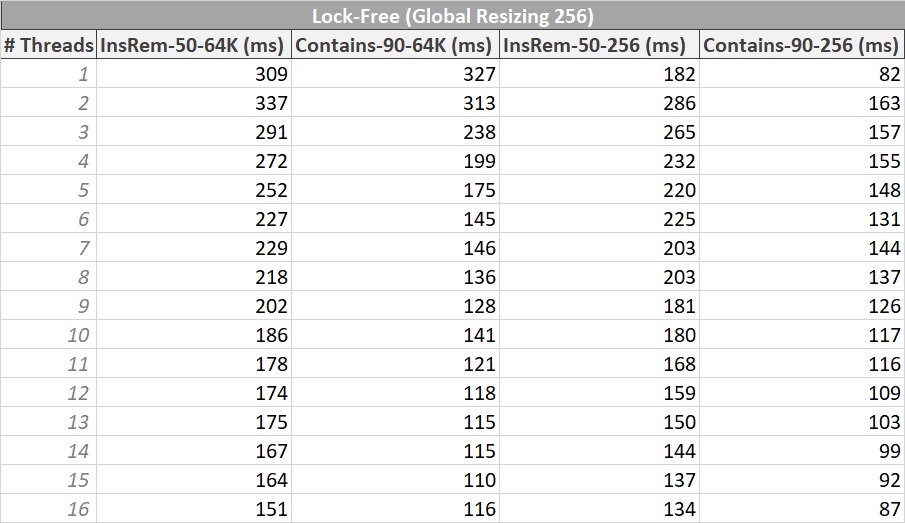
\includegraphics[width=0.5\linewidth]{TableH.png}
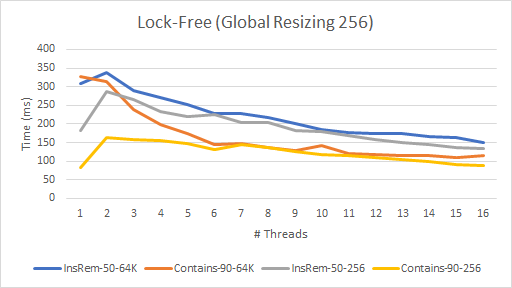
\includegraphics[width=0.5\linewidth]{GraphH.png}
\bigskip
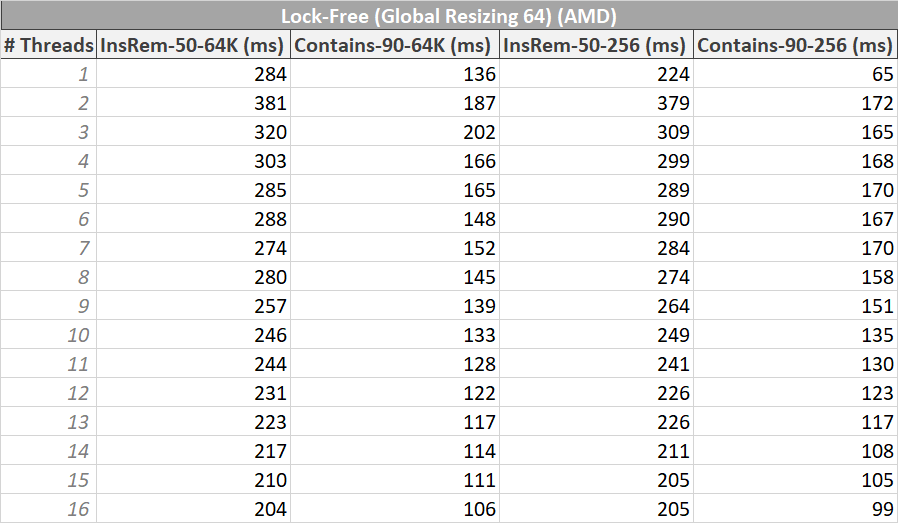
\includegraphics[width=0.5\linewidth]{TableI.png}
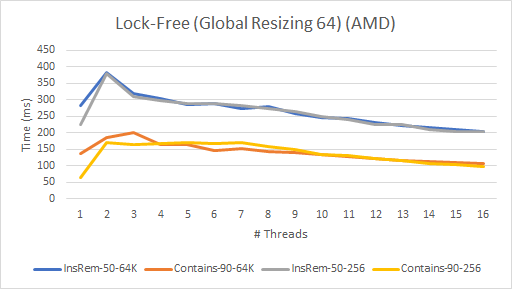
\includegraphics[width=0.5\linewidth]{GraphI.png}


\nocite{*}
\bibliography{bibliography}
\bibliographystyle{IEEEtr}


\end{document}
